\documentclass[aspectratio=169]{beamer} 

\usepackage{hayesmacros}

\usetheme[block=fill]{metropolis}
\setsansfont{Fira Sans}  % be sure to compile with XeLaTeX
% \setmonofont{Fira Mono}  % be sure to compile with XeLaTeX

\usepackage{natbib}
\usepackage{nicematrix}
\usepackage{fontawesome5}
\usepackage{xcolor}

\newtheorem{proposition}{Proposition}
\newtheorem{assumption}{Assumption}
\theoremstyle{remark}
\newtheorem*{remark}{Remark}

\setbeamercolor{background canvas}{bg=white}
\setbeamercolor{normal text}{fg=black}
\setbeamercolor{frametitle}{bg=black, fg=white}

\hypersetup{colorlinks,citecolor=cyan, urlcolor=cyan, linkcolor=black}


\title{Asymptotic unidentifiability of peer effects in the linear-in-means model}
\date{2024-04-04 @ 12:30 pm\\ Service Memorial Institute 133, Medical Sciences Center, UW-Madison}
\author{Alex Hayes | PhD Defense}
\institute{Department of Statistics, University of Wisconsin-Madison}

\begin{document}

\maketitle

% {
%     \usebackgroundtemplate{
\includegraphics[width=\paperwidth]{figures/this_is_fine.jpeg}}
%     \begin{frame}
%     \end{frame}
% }

\begin{frame}{What are peer effects?}
    \begin{columns}
        \column{0.5\textwidth}
        \vspace{7mm}
        
        \textbf{Contagion}: if my friends get sick, I am more likely to set sick
        
        \vspace{4mm}
        
        \textbf{Direct effect}: if I get vaccinated, I am less likely to get sick
        
        \vspace{4mm}
        
        \textbf{Interference}: if my friends get vaccinated, I am less likely to get sick
        
        \vspace{7mm}
        
        {\footnotesize * Not a causal talk. But causally inspired.}
        
        \column{0.5\textwidth}
        \begin{figure}[ht]
            \centering
            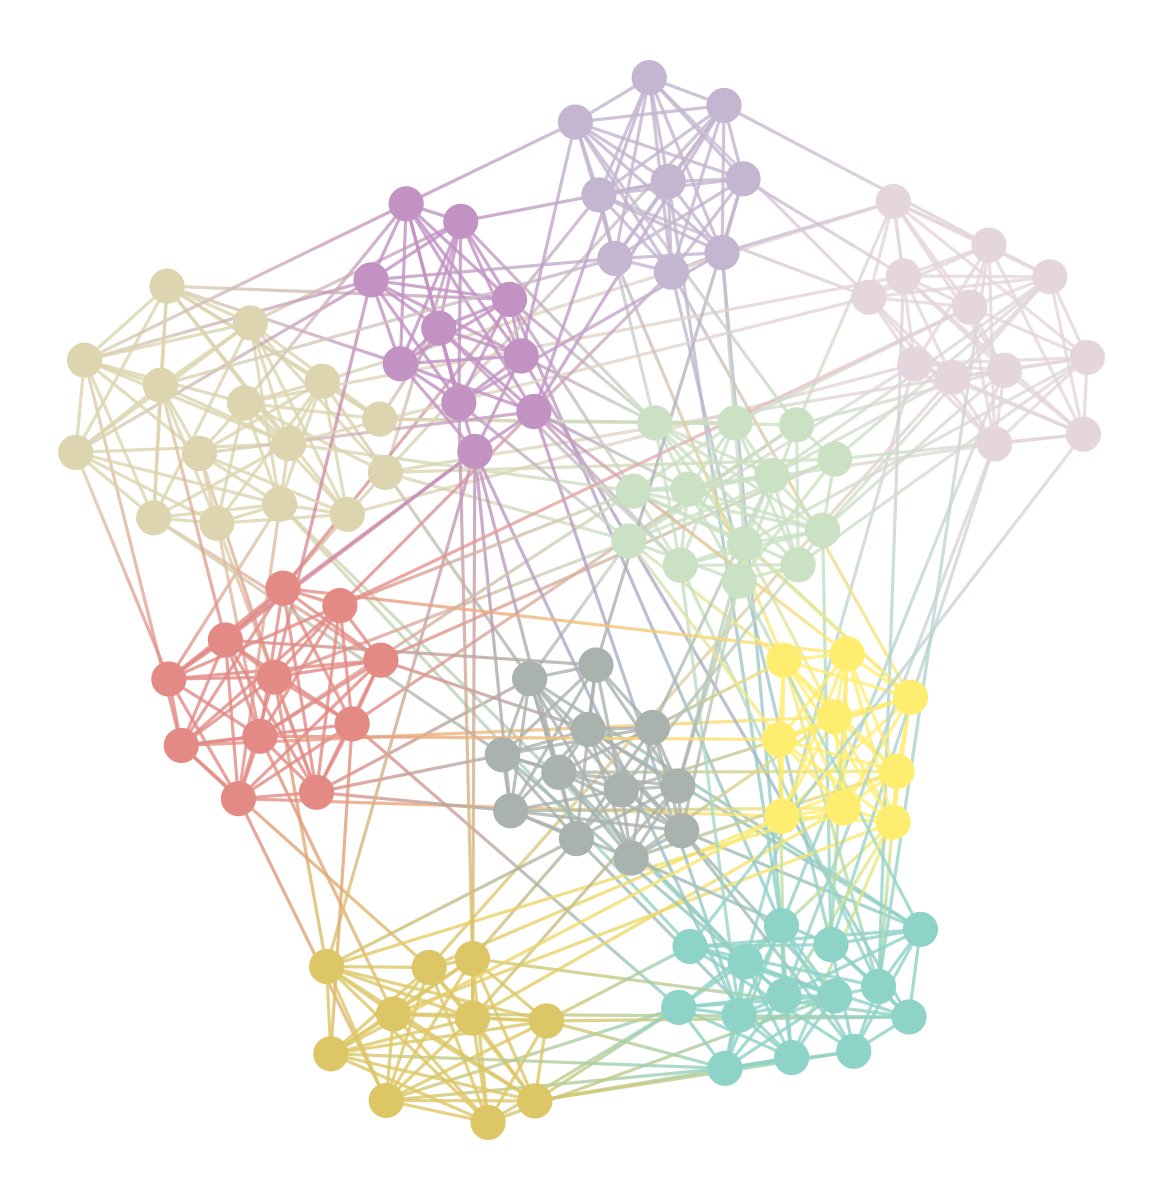
\includegraphics[width=\textwidth]{figures/assortative.png}
        \end{figure}
    \end{columns}
\end{frame}

\begin{frame}{The canonical linear model for peer effects}
    
    \begin{align*}
        \underbrace{Y_i}_\text{sick?} =
        \underbrace{\alpha}_{\substack{\text{base}                                    \\ \text{rate}}} +
        \underbrace{\beta}_{\substack{\text{contagion}                                \\ \text{effect}}}
        \underbrace{\sum_{i \neq j} \frac{A_{ij}}{d_i} Y_j}_{\substack{\text{portion} \\ \text{sick} \\ \text{peers}}} + 
        \underbrace{\gamma}_{\substack{\text{direct}                                  \\ \text{effect}}}
        \underbrace{T_i}_\text{vaccinated?} + 
        \underbrace{\delta}_{\substack{\text{interference}                            \\ \text{effect}}}
        \underbrace{\sum_{i \neq j} \frac{A_{ij}}{d_i} T_j}_{\substack{\text{portion} \\ \text{vaccinated} \\ \text{peers}}} +
        \underbrace{\varepsilon_i}_\text{error}
    \end{align*}
    
    {
    %\footnotesize
    \begin{table}[]
        \begin{tabular}{lcl}
            Outcome          & $Y_i$    & $\in \{0, 1\}$              \\
            Treatment        & $T_i$    & $\in \{0, 1\}$              \\
            Adjacency matrix & $A$      & $\in \{0, 1\}^{n \times n}$ \\
            Edge $i \sim j$  & $A_{ij}$ & $\in \{0, 1\}$              \\
            Node degree      & $d_i$    & $\in \mathbb{Z}^+$          \\
        \end{tabular}
    \end{table}
    }
\end{frame}

\begin{frame}
    \vspace{5mm}
    \begin{figure}
        \centering
        
\includegraphics[width=\textwidth]{figures/manski1993.png}
    \end{figure}
\end{frame}

\begin{frame}{Manski's reflection problem: highly structured networks break the model}
    
    \tikzset{every loop/.style={}}
    
    \begin{columns}
        \begin{column}{0.5\textwidth}
            \begin{figure}
                \centering
                \begin{tikzpicture}
                    \node[shape=circle,draw=black,label=above left:{$T_A = 1$}] (A) at (0,1) {A};
                    \node[shape=circle,draw=black,label=below left:{$T_B = 0$}] (B) at (1,0) {B};
                    \node[shape=circle,draw=black,label=above right:{$T_C = 1$}] (C) at (1.5,1.5) {C};
                    \node[shape=circle,draw=black,label=above right:{$T_D = 1$}] (D) at (2.75,0.5) {D};
                    
                    \path (A) edge [loop above] node {} (A);
                    \path (B) edge [loop below] node {} (B);
                    \path (C) edge [loop above] node {} (C);
                    \path (D) edge [loop above] node {} (D);
                    
                    \draw (A) -- (B);
                    \draw (A) -- (C);
                    \draw (A) -- (D);
                    \draw (B) -- (C);
                    \draw (B) -- (D);
                    \draw (C) -- (D);
                \end{tikzpicture}
            \end{figure}
        \end{column}
        \begin{column}{0.5\textwidth}
            
            Average value of $T$ amongst peers is the same for all nodes!
            
            \begin{align*}
                GT_A & = 3/4  \\
                GT_B & = 3/4  \\
                GT_C & = 3/4  \\
                GT_D & = 3/4
            \end{align*}
            
            \textbf{Problem:} cannot distinguish base rate $\alpha$ from interference effect $\delta$
        \end{column}
    \end{columns}
\end{frame}

\begin{frame}{Manski's reflection problem: highly structured networks break the model}
    
    \tikzset{every loop/.style={}}
    
    \begin{columns}
        \begin{column}{0.5\textwidth}
            \begin{figure}
                \centering
                \begin{tikzpicture}
                    \node[shape=circle,draw=black,label=above left:{$T_A = 1$}] (A) at (0,1) {A};
                    \node[shape=circle,draw=black,label=below left:{$T_B = 0$}] (B) at (1,0) {B};
                    \node[shape=circle,draw=black,label=above right:{$T_C = 1$}] (C) at (1.5,1.5) {C};
                    \node[shape=circle,draw=black,label=above right:{$T_D = 1$}] (D) at (2.75,0.5) {D};
                    
                    \path (A) edge [loop above] node {} (A);
                    \path[] (B) edge [loop below] node {} (B);
                    \path (C) edge [loop above] node {} (C);
                    \path (D) edge [loop above] node {} (D);
                    
                    \draw (A) -- (B);
                    \draw (A) -- (C);
                    \draw (A) -- (D);
                    \draw (B) -- (C);
                    \draw (B) -- (D);
                    \draw (C) -- (D);
                \end{tikzpicture}
            \end{figure}
        \end{column}
        \begin{column}{0.5\textwidth}
            \begin{equation*}
                \begin{bmatrix}
                    Y_A \\
                    Y_B \\
                    Y_C \\
                    Y_D
                \end{bmatrix}
                =
                \underbrace{
                    \begin{bNiceMatrix}[first-row,first-col]
                         & 1_n & GY   & T & GT  \\
                         & 1   & GY_A & 1 & 3/4 \\
                         & 1   & GY_B & 0 & 3/4 \\
                         & 1   & GY_C & 1 & 3/4 \\
                         & 1   & GY_D & 1 & 3/4 \\
                    \end{bNiceMatrix}
                }_W
                \begin{bmatrix}
                    \alpha \\
                    \beta  \\
                    \gamma \\
                    \delta
                \end{bmatrix}
                +
                \begin{bmatrix}
                    \varepsilon_A \\
                    \varepsilon_B \\
                    \varepsilon_C \\
                    \varepsilon_D
                \end{bmatrix}
            \end{equation*}
            
            \textbf{Problem}: Design matrix $W$ becomes collinear!
        \end{column}
    \end{columns}
\end{frame}

\begin{frame}{Identification}
    
    Define the degree matrix $D = \diag(d_1, d_2, \dots, d_n)$, where $d_i = \sum_j A_{ij}$. Let $G = D^{-1} A$ be the row-normalized adjacency matrix. Then
    \begin{equation*} \label{eq:lim-mv}
        Y = \alpha 1_n + \beta G Y + T \gamma + G T \delta + \varepsilon.
    \end{equation*}
    
    \begin{definition}
        We say that $(\alpha, \beta, \gamma, \delta)$ are \emph{identified} when the columns of the design matrix 
        \begin{equation*}
            \label{eq:design}
            W_n = \begin{bmatrix} 1_n & GY & T & GT \end{bmatrix}.
        \end{equation*}
        are linearly independent. Otherwise, we say that $(\alpha, \beta, \gamma, \delta)$ are \emph{unidentified}.
    \end{definition}
    
    We assume that $\mathbb E \left[\varepsilon | W_n \right] = 0$.
\end{frame}

\begin{frame}
    \begin{figure}
        \centering
        
\includegraphics[width=\textwidth]{figures/bramoulle2009.png}
    \end{figure}
\end{frame}

\begin{frame}{Bramoull\'e: intransivity (i.e, open triangles) fixes the problem}
    
    \begin{columns}
        \begin{column}{0.5\textwidth}
            \begin{figure}
                \centering
                \begin{tikzpicture}
                    \node[shape=circle,draw=black] (A) at (0,1) {A};
                    \node[shape=circle,draw=black] (B) at (1,0) {B};
                    \node[shape=circle,draw=black] (C) at (1.5,1.5) {C};
                    \node[shape=circle,draw=black] (D) at (2.75,0.5) {D};
                    
                    \draw (A) -- (B);
                    \draw (A) -- (C);
                    \draw (A) -- (D);
                    \draw (C) -- (D);
                \end{tikzpicture}
            \end{figure}
        \end{column}
        \begin{column}{0.5\textwidth}
            
            $A \leftrightarrow B \leftrightarrow D$ is an intransitive triangle. If $B$ were friends with $D$ it would ``close'' the triangle
            
            \vspace{4mm}
            
            \textbf{Since 2009:} as long as there is intransitive, $(\alpha, \beta, \gamma, \delta)$ are identified, practitioners are good to use the linear-in-means model
            
            \vspace{4mm}
            
            Reflection problem solved!
        \end{column}
    \end{columns}
\end{frame}

\begin{frame}
    \begin{figure}
        \centering
        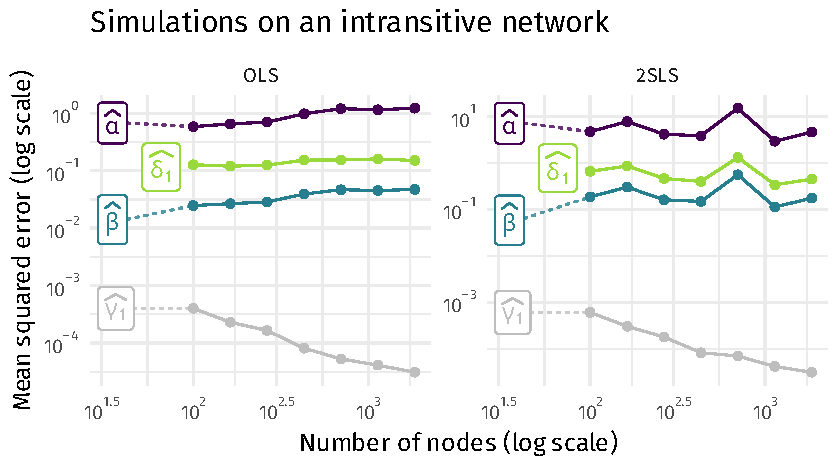
\includegraphics{figures/simulations/defense-mse.pdf}
    \end{figure}
\end{frame}

\begin{frame}
    \begin{figure}
        \centering
        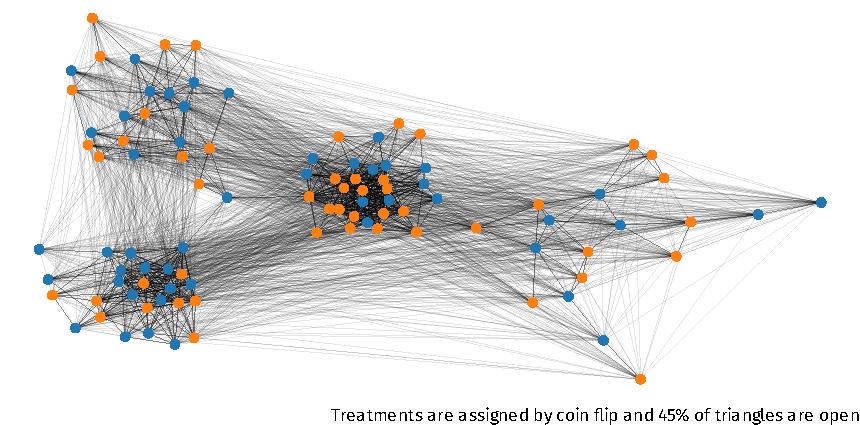
\includegraphics{figures/simulations/defense-backbone.pdf}
    \end{figure}
\end{frame}

% action of G on nodal covariates X
% identification and identification problems
% manski
% bramoulle and intransivity
% doing some simulations, developing an estimator and the results were wonky -- what's happening

\begin{frame}
    Let $G_{ij} = A_{ij} / d_i$ be the row-normalization of $A$. We express the previous model in matrix-vector notation as
    \begin{align*}
        Y & = \alpha 1_n + \beta G Y + \gamma T + \delta G T + \varepsilon
    \end{align*}
    If $\abs{\beta} < 1$, then $I - \beta G$ is invertible and there is a unique solution 
    \begin{align*}
        Y & = \paren*{I - \beta G}^{-1} \paren*{\alpha 1_n + \gamma T + \delta G T + \varepsilon}                                                                                \\
          & = \sum_{k=0}^\infty \beta^k G^k \paren*{\alpha 1_n + \gamma T + \delta G T + \varepsilon} & \text{since } \paren*{I - \beta G}^{-1} = \sum_{k=0}^\infty \beta^k G^k
    \end{align*}
\end{frame}

\begin{frame}
    \begin{columns}
        \begin{column}{0.5\textwidth}
            \begin{figure}
                \centering
                \begin{tikzpicture}
                    \node[shape=circle,draw=black,label=above left:A] (A) at (0,1) {1};
                    \node[shape=circle,draw=black,label=below left:B] (B) at (1,0) {0};
                    \node[shape=circle,draw=black,label=above right:C] (C) at (1.5,1.5) {1};
                    \node[shape=circle,draw=black,label=above right:D] (D) at (2.75,0.5) {1};
                    
                    \draw (A) -- (B);
                    \draw (A) -- (C);
                    \draw (B) -- (C);
                    \draw (C) -- (D);
                \end{tikzpicture}
                \caption{$T$}
            \end{figure}
        \end{column}
        \begin{column}{0.5\textwidth}
            \begin{figure}
                \centering
                \begin{tikzpicture}
                    \node[shape=circle,draw=black,label=above left:A] (A) at (0,1) {$\frac 12$};
                    \node[shape=circle,draw=black,label=below left:B] (B) at (1,0) {1};
                    \node[shape=circle,draw=black,label=above right:C] (C) at (1.5,1.5) {$\frac 23$};
                    \node[shape=circle,draw=black,label=above right:D] (D) at (2.75,0.5) {1};
                    
                    \draw (A) -- (B);
                    \draw (A) -- (C);
                    \draw (B) -- (C);
                    \draw (C) -- (D);
                \end{tikzpicture}
                \caption{$GT$}
            \end{figure}
        \end{column}
    \end{columns}
\end{frame}

\begin{frame}
    \begin{proposition}[Finite sample identification, \cite{bramoulle2009}]
        Let $\varepsilon$ be mean zero, i.i.d. noise and let
        \begin{align*}
            Y & = \alpha 1_n + \beta G Y + \gamma T + \delta G T + \varepsilon                        
        \end{align*}
        Suppose that $\abs{\beta} < 1$ and $\gamma \beta + \delta \neq 0$. If $I, G$ and $G^2$ are linearly independent, in the sense that $a I + b G + c G^2 = 0$ requires $a = b = c = 0$, then $\alpha, \beta, \gamma$ and $\delta$ are identified.
    \end{proposition}
    
    $\gamma \beta + \delta \neq 0$ means that there is either some interference effect, or some direct effect and some contagion effect, and if there are both, they don't cancel each other out.
\end{frame}

\begin{frame}
    \begin{proposition}
        If $\gamma \beta + \delta \neq 0$ and $G$ has three or more distinct eigenvalues, then $\alpha, \beta, \gamma$ and $\delta$ are identified.
    \end{proposition}
    
    Promising! If $G$ is from a stochastic blockmodel, identification likely.
\end{frame}

\begin{frame}{Disappearing asymptotic identification: a simple case \citep{li2022c}}
    \begin{align*}
        \underbrace{Y_i}_\text{sick?} =
        \underbrace{\alpha}_{\substack{\text{base}                                    \\ \text{rate}}} +
        \underbrace{\gamma}_{\substack{\text{direct}                                  \\ \text{effect}}}
        \underbrace{T_i}_\text{vaccinated?} + 
        \underbrace{\delta}_{\substack{\text{interference}                            \\ \text{effect}}}
        \underbrace{\sum_{i \neq j} \frac{A_{ij}}{d_i} T_j}_{\substack{\text{portion} \\ \text{vaccinated} \\ \text{peers}}} +
        \underbrace{\varepsilon_i}_\text{error}
    \end{align*}
    
    Problem: $GT$ term converges to a constant
    
    \begin{align*}
        \sum_{i \neq j} \frac{A_{ij}}{d_i} T_j \to \pi                         
    \end{align*}
\end{frame}

\begin{frame}{$GY$ can also be a problem}
    Suppose no node is isolated (otherwise the intercept differs for isolated and connected nodes in reduced form) then the reduced form of $Y$ is given by
    \begin{align*}
        Y & = \frac{\alpha}{1 - \beta} 1_n  + \gamma T + (\gamma \beta + \delta) \sum_{k=0}^\infty \beta^k G^{k+1} T + \sum_{k=0}^\infty \beta^k G^k \varepsilon
    \end{align*}
    then
    \begin{align*}
        GY = 
        \frac{\alpha}{1 - \beta} 1_n + 
        \underbrace{\gamma G T}_{\substack{\text{neighborhood}                                              \\ \text{average}}} + 
        \underbrace{(\gamma \beta + \delta) \sum_{k=0}^\infty \beta^k G^{k+2} T}_{\substack{\text{repeated} \\ \text{neighborhood} \\ \text{averages}}} +
        \underbrace{\sum_{k=0}^\infty \beta^k G^{k+1} \varepsilon}_{\substack{\text{neighborhood}           \\ \text{repeated} \\ \text{averages}}}
    \end{align*}
\end{frame}

\begin{frame}
    \begin{align*}
        GY = 
        \frac{\alpha}{1 - \beta} 1_n + 
        \underbrace{\gamma G T}_{\substack{\text{neighborhood}                                              \\ \text{average}}} + 
        \underbrace{(\gamma \beta + \delta) \sum_{k=0}^\infty \beta^k G^{k+2} T}_{\substack{\text{repeated} \\ \text{neighborhood} \\ \text{averages}}} +
        \underbrace{\sum_{k=0}^\infty \beta^k G^{k+1} \varepsilon}_{\substack{\text{neighborhood}           \\ \text{repeated} \\ \text{averages}}}
    \end{align*}
    If neighborhood averages $GT$ are converging, repeated neighborhood averages converge as well\footnote{Possibly under suitable conditions}, because $G 1_n = 1_n$ (neighborhood average of constants is constant)
\end{frame}

\begin{frame}
    Roughly, if
    \begin{enumerate}
        \item neighborhoods $d_i$ are all getting larger in $n$, and
        \item there is no CLT/LLN breaking strong dependence between network $A$ and nodal covariate $T$
    \end{enumerate}
    Then 
    \begin{align*}
        \lim_{n \to \infty} GT & \to C  & C \in \R   \\
        \lim_{n \to \infty} GY & \to C' & C' \in \R
    \end{align*}
    
    \textbf{Then contagion and interference effects are the same for everyone, and indistinguishable from base rates}
    
    The direct effect $\gamma$ is still identified.
\end{frame}

\begin{frame}
    \begin{theorem}[Identification failure when $T$ independent of $A$]
        Let $\varepsilon$ be mean zero, i.i.d. noise and let
        \begin{align*}
            Y & = \alpha 1_n + \beta G Y + \gamma T + \delta G T + \varepsilon                        
        \end{align*}
        Suppose $\abs{\beta} < 1$. If $T$ is sub-gamma and independent of the network $A$, and $\min_{i \in [n]} d_i = \omega(\log n)$, then there exists constants $C, C' \in \R$ such that
        \begin{align*}
            \lim_{n \to \infty} \sup_{i \in [n]} \abs*{GT - 1_n C}  & = \op{1},  & \text{and} \\
            \lim_{n \to \infty} \sup_{i \in [n]} \abs*{GY - 1_n C'} & = \op{1}.
        \end{align*}
    \end{theorem}
    
    \footnotesize * This covers fixed networks and conditioning on the network
\end{frame}

\begin{frame}
    \begin{theorem}[Identification failure in random dot product graphs]
        Let $\varepsilon$ be mean zero, i.i.d. noise and let
        \begin{align*}
            Y & = \alpha 1_n + \beta G Y + \gamma T + \delta G T + \varepsilon                        
        \end{align*}
        Suppose $\abs{\beta} < 1$. Let $(A, \X) \sim \text{RDPG}(F, n)$ and let $T = \X \in \R^{n \times d}$. Then there exists constants $C, C' \in \R^d$ such that
        \begin{align*}
            \lim_{n \to \infty} \sup_{i \in [n]} \abs*{GT - 1_n C}  & = \op{1},  & \text{and} \\
            \lim_{n \to \infty} \sup_{i \in [n]} \abs*{GY - 1_n C'} & = \op{1}.
        \end{align*}
    \end{theorem}
\end{frame}

\begin{frame}{Why this matters}
    
    \begin{enumerate}
        \item \cite{shalizi2011,mcfowland2021}: homophily and contagion are non-parametrically confounded. Must make parametric assumptions to estimate contagion effects.
        \item \cite{bramoulle2020}: most parametric contagion identification theory considers fixed $n$ setting but not the $n \to \infty$ limit. Many results won't hold under stochastic blockmodels.
    \end{enumerate}
\end{frame}

\begin{frame}{Open questions}
    
    \begin{itemize}
        \item Do $GT$ and $GY$ ever not converge to constants?
        \item Are longitudinal contagion models also affected?
        \item What happens in sparse networks asymptotically?
    \end{itemize}
\end{frame}

\begin{frame}{Thank you! Questions?}
    
    \textbf{Stay in touch}
    
    \begin{itemize}
        \item[] \faIcon{twitter} \href{https://twitter.com/alexpghayes}{@alexpghayes}
        \item[] \faIcon[regular]{envelope} \href{mailto:alex.hayes@wisc.edu}{alex.hayes@wisc.edu}
        \item[] \faIcon{wordpress} \url{https://www.alexpghayes.com}
        \item[] \faIcon{github} \url{https://github.com/alexpghayes}
    \end{itemize}
    
\end{frame}

\appendix

\bibliographystyle{chicago}
\bibliography{references}

\end{document}